\chapter{Consultas em Árvores}

\index{tree query}

Este capítulo aborda técnicas para processar consultas em subárvores e caminhos de uma árvore enraizada. Por exemplo, algumas dessas consultas são:

\begin{itemize}
\item Qual é o $k$-ésimo ancestral de um nó?
\item Qual é a soma dos valores na subárvore de um nó?
\item Qual é a soma dos valores em um caminho entre dois nós?
\item Qual é o ancestral comum mais baixo de dois nós?
\end{itemize}

\section{Encontrando Ancestrais}

\index{ancestor}

O $k$-ésimo \key{ancestral} de um nó $x$ em uma árvore enraizada é o nó que alcançaremos se subirmos $k$ níveis a partir de $x$. Seja $\texttt{ancestral}(x,k)$ o $k$-ésimo ancestral de um nó $x$ (ou $0$ se não houver tal ancestral). Por exemplo, na árvore a seguir,
$\texttt{ancestral}(2,1)=1$ e $\texttt{ancestral}(8,2)=4$.

\begin{center}
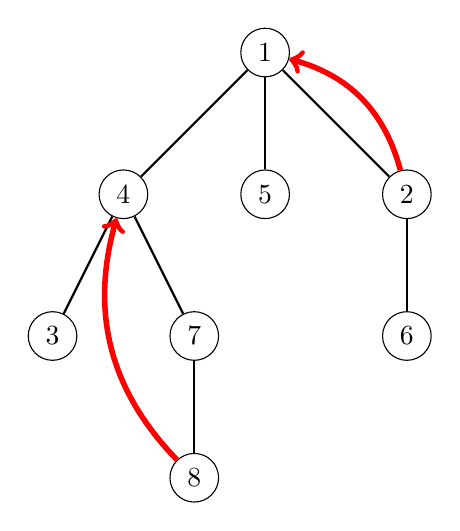
\begin{tikzpicture}[scale=0.9]
\node[draw, circle] (1) at (0,3) {$1$};
\node[draw, circle] (2) at (2,1) {$2$};
\node[draw, circle] (3) at (-2,1) {$4$};
\node[draw, circle] (4) at (0,1) {$5$};
\node[draw, circle] (5) at (2,-1) {$6$};
\node[draw, circle] (6) at (-3,-1) {$3$};
\node[draw, circle] (7) at (-1,-1) {$7$};
\node[draw, circle] (8) at (-1,-3) {$8$};
\path[draw,thick,-] (1) -- (2);
\path[draw,thick,-] (1) -- (3);
\path[draw,thick,-] (1) -- (4);
\path[draw,thick,-] (2) -- (5);
\path[draw,thick,-] (3) -- (6);
\path[draw,thick,-] (3) -- (7);
\path[draw,thick,-] (7) -- (8);

\path[draw=red,thick,->,line width=2pt] (8) edge [bend left] (3);
\path[draw=red,thick,->,line width=2pt] (2) edge [bend right] (1);
\end{tikzpicture}
\end{center}

Uma maneira fácil de calcular qualquer valor de $\texttt{ancestral}(x,k)$ é realizar uma sequência de $k$ movimentos na árvore. No entanto, a complexidade de tempo deste método é $O(k)$, o que pode ser lento, pois uma árvore de $n$ nós pode ter uma cadeia de $n$ nós.

Felizmente, usando uma técnica semelhante àquela utilizada no Capítulo 16.3, qualquer valor de $\texttt{ancestral}(x,k)$ pode ser calculado eficientemente em tempo $O(\log k)$ após o pré-processamento. A ideia é pré-calcular todos os valores $\texttt{ancestral}(x,k)$ onde $k \le n$ é uma potência de dois. Por exemplo, os valores para a árvore acima são os seguintes:

\begin{center}
\begin{tabular}{r|rrrrrrrrr}
$x$ & 1 & 2 & 3 & 4 & 5 & 6 & 7 & 8 \\
\hline
$\texttt{ancestral}(x,1)$ & 0 & 1 & 4 & 1 & 1 & 2 & 4 & 7 \\
$\texttt{ancestral}(x,2)$ & 0 & 0 & 1 & 0 & 0 & 1 & 1 & 4 \\
$\texttt{ancestral}(x,4)$ & 0 & 0 & 0 & 0 & 0 & 0 & 0 & 0 \\
$\cdots$ \\
\end{tabular}
\end{center}

O pré-processamento leva tempo $O(n \log n)$, pois $O(\log n)$ valores são calculados para cada nó. Após isso, qualquer valor de $\texttt{ancestral}(x,k)$ pode ser calculado em tempo $O(\log k)$ representando $k$ como uma soma onde cada termo é uma potência de dois.

\section{Subárvores e Caminhos}

\index{tree traversal array}

Um \key{vetor de percurso de árvore} contém os nós de uma árvore enraizada na ordem em que uma busca em profundidade a partir do nó raiz os visita. Por exemplo, na árvore:

\begin{center}
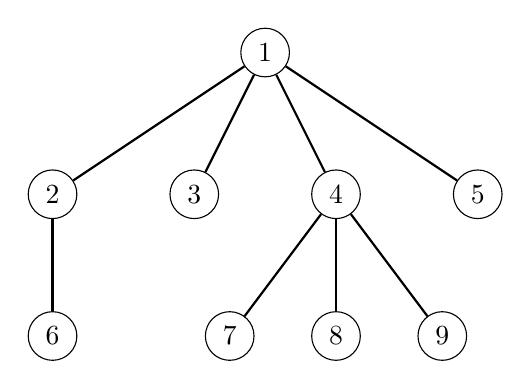
\begin{tikzpicture}[scale=0.9]
\node[draw, circle] (1) at (0,3) {$1$};
\node[draw, circle] (2) at (-3,1) {$2$};
\node[draw, circle] (3) at (-1,1) {$3$};
\node[draw, circle] (4) at (1,1) {$4$};
\node[draw, circle] (5) at (3,1) {$5$};
\node[draw, circle] (6) at (-3,-1) {$6$};
\node[draw, circle] (7) at (-0.5,-1) {$7$};
\node[draw, circle] (8) at (1,-1) {$8$};
\node[draw, circle] (9) at (2.5,-1) {$9$};

\path[draw,thick,-] (1) -- (2);
\path[draw,thick,-] (1) -- (3);
\path[draw,thick,-] (1) -- (4);
\path[draw,thick,-] (1) -- (5);
\path[draw,thick,-] (2) -- (6);
\path[draw,thick,-] (4) -- (7);
\path[draw,thick,-] (4) -- (8);
\path[draw,thick,-] (4) -- (9);
\end{tikzpicture}
\end{center}

Uma busca em profundidade procede da seguinte forma:

\begin{center}
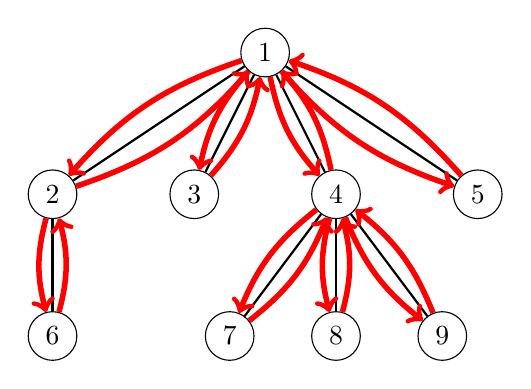
\begin{tikzpicture}[scale=0.9]
\node[draw, circle] (1) at (0,3) {$1$};
\node[draw, circle] (2) at (-3,1) {$2$};
\node[draw, circle] (3) at (-1,1) {$3$};
\node[draw, circle] (4) at (1,1) {$4$};
\node[draw, circle] (5) at (3,1) {$5$};
\node[draw, circle] (6) at (-3,-1) {$6$};
\node[draw, circle] (7) at (-0.5,-1) {$7$};
\node[draw, circle] (8) at (1,-1) {$8$};
\node[draw, circle] (9) at (2.5,-1) {$9$};

\path[draw,thick,-] (1) -- (2);
\path[draw,thick,-] (1) -- (3);
\path[draw,thick,-] (1) -- (4);
\path[draw,thick,-] (1) -- (5);
\path[draw,thick,-] (2) -- (6);
\path[draw,thick,-] (4) -- (7);
\path[draw,thick,-] (4) -- (8);
\path[draw,thick,-] (4) -- (9);


\path[draw=red,thick,->,line width=2pt] (1) edge [bend right=15] (2);
\path[draw=red,thick,->,line width=2pt] (2) edge [bend right=15] (6);
\path[draw=red,thick,->,line width=2pt] (6) edge [bend right=15] (2);
\path[draw=red,thick,->,line width=2pt] (2) edge [bend right=15] (1);
\path[draw=red,thick,->,line width=2pt] (1) edge [bend right=15] (3);
\path[draw=red,thick,->,line width=2pt] (3) edge [bend right=15] (1);
\path[draw=red,thick,->,line width=2pt] (1) edge [bend right=15] (4);
\path[draw=red,thick,->,line width=2pt] (4) edge [bend right=15] (7);
\path[draw=red,thick,->,line width=2pt] (7) edge [bend right=15] (4);
\path[draw=red,thick,->,line width=2pt] (4) edge [bend right=15] (8);
\path[draw=red,thick,->,line width=2pt] (8) edge [bend right=15] (4);
\path[draw=red,thick,->,line width=2pt] (4) edge [bend right=15] (9);
\path[draw=red,thick,->,line width=2pt] (9) edge [bend right=15] (4);
\path[draw=red,thick,->,line width=2pt] (4) edge [bend right=15] (1);
\path[draw=red,thick,->,line width=2pt] (1) edge [bend right=15] (5);
\path[draw=red,thick,->,line width=2pt] (5) edge [bend right=15] (1);

\end{tikzpicture}
\end{center}

Portanto, o vetor de percurso de árvore correspondente é o seguinte:

\begin{center}
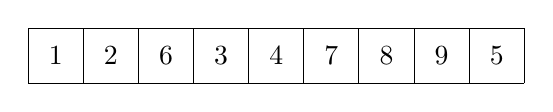
\begin{tikzpicture}[scale=0.7]
\draw (0,0) grid (9,1);

\node at (0.5,0.5) {$1$};
\node at (1.5,0.5) {$2$};
\node at (2.5,0.5) {$6$};
\node at (3.5,0.5) {$3$};
\node at (4.5,0.5) {$4$};
\node at (5.5,0.5) {$7$};
\node at (6.5,0.5) {$8$};
\node at (7.5,0.5) {$9$};
\node at (8.5,0.5) {$5$};
\end{tikzpicture}
\end{center}

\subsubsection{Consultas em Subárvores}

Cada subárvore de uma árvore corresponde a um subvetor do vetor de percurso de árvore, de forma que o primeiro elemento do subvetor é o nó raiz. Por exemplo, o seguinte subvetor contém os nós da subárvore do nó $4$:

\begin{center}
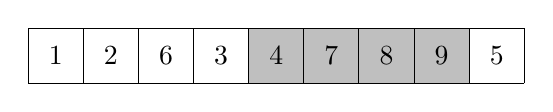
\begin{tikzpicture}[scale=0.7]
\fill[color=lightgray] (4,0) rectangle (8,1);
\draw (0,0) grid (9,1);

\node at (0.5,0.5) {$1$};
\node at (1.5,0.5) {$2$};
\node at (2.5,0.5) {$6$};
\node at (3.5,0.5) {$3$};
\node at (4.5,0.5) {$4$};
\node at (5.5,0.5) {$7$};
\node at (6.5,0.5) {$8$};
\node at (7.5,0.5) {$9$};
\node at (8.5,0.5) {$5$};
\end{tikzpicture}
\end{center}

Usando esse fato, podemos processar eficientemente consultas relacionadas a subárvores de uma árvore. Como exemplo, considere um problema onde cada nó recebe um valor e nossa tarefa é oferecer suporte às seguintes consultas:

\begin{itemize}
\item atualizar o valor de um nó
\item calcular a soma dos valores na subárvore de um nó
\end{itemize}

Considere a seguinte árvore onde os números azuis são os valores dos nós. Por exemplo, a soma da subárvore do nó $4$ é $3+4+3+1=11$.

\begin{center}
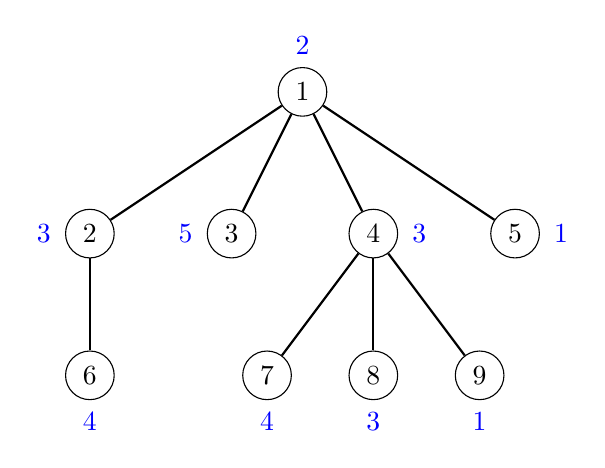
\begin{tikzpicture}[scale=0.9]
\node[draw, circle] (1) at (0,3) {$1$};
\node[draw, circle] (2) at (-3,1) {$2$};
\node[draw, circle] (3) at (-1,1) {$3$};
\node[draw, circle] (4) at (1,1) {$4$};
\node[draw, circle] (5) at (3,1) {$5$};
\node[draw, circle] (6) at (-3,-1) {$6$};
\node[draw, circle] (7) at (-0.5,-1) {$7$};
\node[draw, circle] (8) at (1,-1) {$8$};
\node[draw, circle] (9) at (2.5,-1) {$9$};

\path[draw,thick,-] (1) -- (2);
\path[draw,thick,-] (1) -- (3);
\path[draw,thick,-] (1) -- (4);
\path[draw,thick,-] (1) -- (5);
\path[draw,thick,-] (2) -- (6);
\path[draw,thick,-] (4) -- (7);
\path[draw,thick,-] (4) -- (8);
\path[draw,thick,-] (4) -- (9);

\node[color=blue] at (0,3+0.65) {2};
\node[color=blue] at (-3-0.65,1) {3};
\node[color=blue] at (-1-0.65,1) {5};
\node[color=blue] at (1+0.65,1) {3};
\node[color=blue] at (3+0.65,1) {1};
\node[color=blue] at (-3,-1-0.65) {4};
\node[color=blue] at (-0.5,-1-0.65) {4};
\node[color=blue] at (1,-1-0.65) {3};
\node[color=blue] at (2.5,-1-0.65) {1};
\end{tikzpicture}
\end{center}

A ideia é construir um vetor de percurso de árvore que contém três valores para cada nó: o identificador do nó, o tamanho da subárvore e o valor do nó. Por exemplo, o vetor para a árvore acima é o seguinte:

\begin{center}
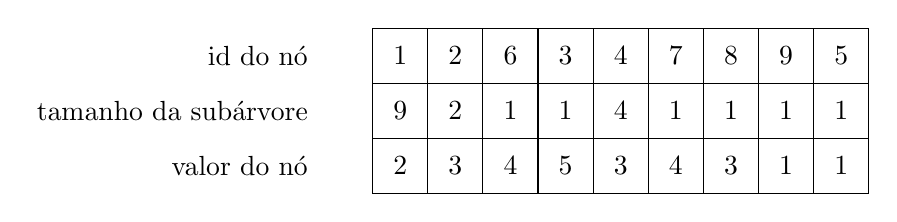
\begin{tikzpicture}[scale=0.7]
\draw (0,1) grid (9,-2);

\node[left] at (-1,0.5) {id do nó};
\node[left] at (-1,-0.5) {tamanho da subárvore};
\node[left] at (-1,-1.5) {valor do nó};

\node at (0.5,0.5) {$1$};
\node at (1.5,0.5) {$2$};
\node at (2.5,0.5) {$6$};
\node at (3.5,0.5) {$3$};
\node at (4.5,0.5) {$4$};
\node at (5.5,0.5) {$7$};
\node at (6.5,0.5) {$8$};
\node at (7.5,0.5) {$9$};
\node at (8.5,0.5) {$5$};

\node at (0.5,-0.5) {$9$};
\node at (1.5,-0.5) {$2$};
\node at (2.5,-0.5) {$1$};
\node at (3.5,-0.5) {$1$};
\node at (4.5,-0.5) {$4$};
\node at (5.5,-0.5) {$1$};
\node at (6.5,-0.5) {$1$};
\node at (7.5,-0.5) {$1$};
\node at (8.5,-0.5) {$1$};

\node at (0.5,-1.5) {$2$};
\node at (1.5,-1.5) {$3$};
\node at (2.5,-1.5) {$4$};
\node at (3.5,-1.5) {$5$};
\node at (4.5,-1.5) {$3$};
\node at (5.5,-1.5) {$4$};
\node at (6.5,-1.5) {$3$};
\node at (7.5,-1.5) {$1$};
\node at (8.5,-1.5) {$1$};
\end{tikzpicture}
\end{center}

Usando este vetor, podemos calcular a soma dos valores em qualquer subárvore primeiro descobrindo o tamanho da subárvore e depois os valores dos nós correspondentes. Por exemplo, os valores na subárvore do nó $4$ podem ser encontrados da seguinte forma:

\begin{center}
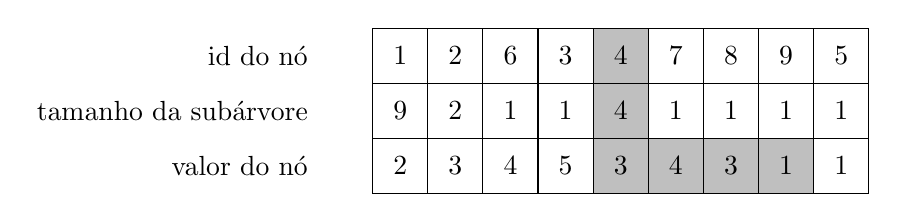
\begin{tikzpicture}[scale=0.7]
\fill[color=lightgray] (4,1) rectangle (5,0);
\fill[color=lightgray] (4,0) rectangle (5,-1);
\fill[color=lightgray] (4,-1) rectangle (8,-2);
\draw (0,1) grid (9,-2);

\node[left] at (-1,0.5) {id do nó};
\node[left] at (-1,-0.5) {tamanho da subárvore};
\node[left] at (-1,-1.5) {valor do nó};

\node at (0.5,0.5) {$1$};
\node at (1.5,0.5) {$2$};
\node at (2.5,0.5) {$6$};
\node at (3.5,0.5) {$3$};
\node at (4.5,0.5) {$4$};
\node at (5.5,0.5) {$7$};
\node at (6.5,0.5) {$8$};
\node at (7.5,0.5) {$9$};
\node at (8.5,0.5) {$5$};

\node at (0.5,-0.5) {$9$};
\node at (1.5,-0.5) {$2$};
\node at (2.5,-0.5) {$1$};
\node at (3.5,-0.5) {$1$};
\node at (4.5,-0.5) {$4$};
\node at (5.5,-0.5) {$1$};
\node at (6.5,-0.5) {$1$};
\node at (7.5,-0.5) {$1$};
\node at (8.5,-0.5) {$1$};

\node at (0.5,-1.5) {$2$};
\node at (1.5,-1.5) {$3$};
\node at (2.5,-1.5) {$4$};
\node at (3.5,-1.5) {$5$};
\node at (4.5,-1.5) {$3$};
\node at (5.5,-1.5) {$4$};
\node at (6.5,-1.5) {$3$};
\node at (7.5,-1.5) {$1$};
\node at (8.5,-1.5) {$1$};
\end{tikzpicture}
\end{center}

Para responder às consultas de forma eficiente, basta armazenar os valores dos nós em uma árvore binária indexada ou árvore de segmentos. Depois disso, podemos atualizar um valor e calcular a soma dos valores em tempo $O(\log n)$.

\subsubsection{Consultas em Caminhos}

Usando um vetor de percurso de árvore, também podemos calcular eficientemente somas de valores em caminhos do nó raiz para qualquer nó da árvore. Considere um problema em que nossa tarefa é oferecer suporte às seguintes consultas:

\begin{itemize}
\item alterar o valor de um nó
\item calcular a soma dos valores em um caminho da raiz até um nó
\end{itemize}

Por exemplo, na árvore a seguir, a soma dos valores do nó raiz ao nó 7 é $4+5+5=14$:

\begin{center}
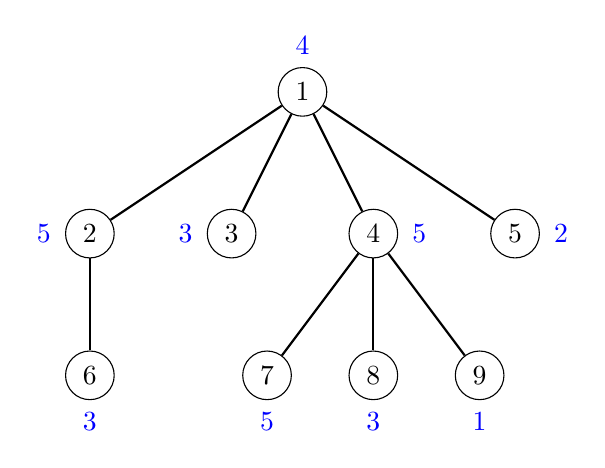
\begin{tikzpicture}[scale=0.9]
\node[draw, circle] (1) at (0,3) {$1$};
\node[draw, circle] (2) at (-3,1) {$2$};
\node[draw, circle] (3) at (-1,1) {$3$};
\node[draw, circle] (4) at (1,1) {$4$};
\node[draw, circle] (5) at (3,1) {$5$};
\node[draw, circle] (6) at (-3,-1) {$6$};
\node[draw, circle] (7) at (-0.5,-1) {$7$};
\node[draw, circle] (8) at (1,-1) {$8$};
\node[draw, circle] (9) at (2.5,-1) {$9$};

\path[draw,thick,-] (1) -- (2);
\path[draw,thick,-] (1) -- (3);
\path[draw,thick,-] (1) -- (4);
\path[draw,thick,-] (1) -- (5);
\path[draw,thick,-] (2) -- (6);
\path[draw,thick,-] (4) -- (7);
\path[draw,thick,-] (4) -- (8);
\path[draw,thick,-] (4) -- (9);

\node[color=blue] at (0,3+0.65) {4};
\node[color=blue] at (-3-0.65,1) {5};
\node[color=blue] at (-1-0.65,1) {3};
\node[color=blue] at (1+0.65,1) {5};
\node[color=blue] at (3+0.65,1) {2};
\node[color=blue] at (-3,-1-0.65) {3};
\node[color=blue] at (-0.5,-1-0.65) {5};
\node[color=blue] at (1,-1-0.65) {3};
\node[color=blue] at (2.5,-1-0.65) {1};
\end{tikzpicture}
\end{center}

Podemos resolver este problema como antes, mas agora cada valor na última linha do vetor é a soma dos valores em um caminho da raiz até o nó. Por exemplo, o seguinte vetor corresponde à árvore acima:

\begin{center}
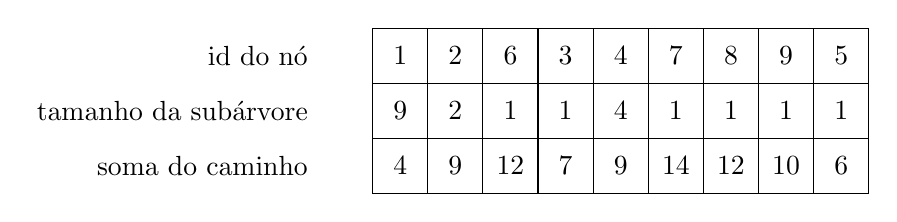
\begin{tikzpicture}[scale=0.7]
\draw (0,1) grid (9,-2);

\node[left] at (-1,0.5) {id do nó};
\node[left] at (-1,-0.5) {tamanho da subárvore};
\node[left] at (-1,-1.5) {soma do caminho};

\node at (0.5,0.5) {$1$};
\node at (1.5,0.5) {$2$};
\node at (2.5,0.5) {$6$};
\node at (3.5,0.5) {$3$};
\node at (4.5,0.5) {$4$};
\node at (5.5,0.5) {$7$};
\node at (6.5,0.5) {$8$};
\node at (7.5,0.5) {$9$};
\node at (8.5,0.5) {$5$};

\node at (0.5,-0.5) {$9$};
\node at (1.5,-0.5) {$2$};
\node at (2.5,-0.5) {$1$};
\node at (3.5,-0.5) {$1$};
\node at (4.5,-0.5) {$4$};
\node at (5.5,-0.5) {$1$};
\node at (6.5,-0.5) {$1$};
\node at (7.5,-0.5) {$1$};
\node at (8.5,-0.5) {$1$};

\node at (0.5,-1.5) {$4$};
\node at (1.5,-1.5) {$9$};
\node at (2.5,-1.5) {$12$};
\node at (3.5,-1.5) {$7$};
\node at (4.5,-1.5) {$9$};
\node at (5.5,-1.5) {$14$};
\node at (6.5,-1.5) {$12$};
\node at (7.5,-1.5) {$10$};
\node at (8.5,-1.5) {$6$};
\end{tikzpicture}
\end{center}

Quando o valor de um nó aumenta em $x$, as somas de todos os nós em sua subárvore aumentam em $x$. Por exemplo, se o valor do nó 4 aumentar em 1, o vetor muda da seguinte forma:

\begin{center}
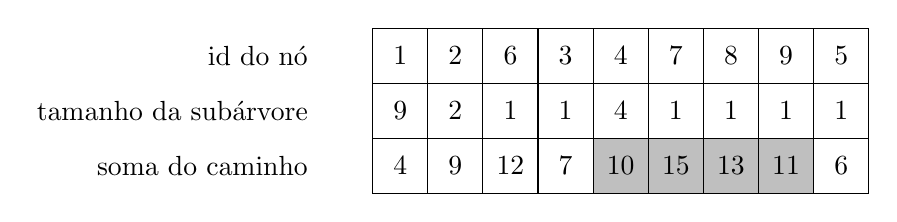
\begin{tikzpicture}[scale=0.7]
\fill[color=lightgray] (4,-1) rectangle (8,-2);
\draw (0,1) grid (9,-2);

\node[left] at (-1,0.5) {id do nó};
\node[left] at (-1,-0.5) {tamanho da subárvore};
\node[left] at (-1,-1.5) {soma do caminho};

\node at (0.5,0.5) {$1$};
\node at (1.5,0.5) {$2$};
\node at (2.5,0.5) {$6$};
\node at (3.5,0.5) {$3$};
\node at (4.5,0.5) {$4$};
\node at (5.5,0.5) {$7$};
\node at (6.5,0.5) {$8$};
\node at (7.5,0.5) {$9$};
\node at (8.5,0.5) {$5$};

\node at (0.5,-0.5) {$9$};
\node at (1.5,-0.5) {$2$};
\node at (2.5,-0.5) {$1$};
\node at (3.5,-0.5) {$1$};
\node at (4.5,-0.5) {$4$};
\node at (5.5,-0.5) {$1$};
\node at (6.5,-0.5) {$1$};
\node at (7.5,-0.5) {$1$};
\node at (8.5,-0.5) {$1$};

\node at (0.5,-1.5) {$4$};
\node at (1.5,-1.5) {$9$};
\node at (2.5,-1.5) {$12$};
\node at (3.5,-1.5) {$7$};
\node at (4.5,-1.5) {$10$};
\node at (5.5,-1.5) {$15$};
\node at (6.5,-1.5) {$13$};
\node at (7.5,-1.5) {$11$};
\node at (8.5,-1.5) {$6$};
\end{tikzpicture}
\end{center}

Assim, para oferecer suporte a ambas as operações, devemos ser capazes de aumentar todos os valores em um intervalo e recuperar um único valor. Isso pode ser feito em tempo $O(\log n)$ usando uma árvore de índice binário ou árvore de segmentos (consulte o Capítulo 9.4).

\section{Ancestral Comum Mais Baixo}

\index{lowest common ancestor}

O \key{ancestral comum mais baixo} de dois nós de uma árvore enraizada é o nó mais baixo cuja subárvore contém ambos os nós. Um problema típico é processar eficientemente consultas que pedem para encontrar o ancestral comum mais baixo de dois nós.

Por exemplo, na árvore a seguir, o ancestral comum mais baixo dos nós 5 e 8 é o nó 2:

\begin{center}
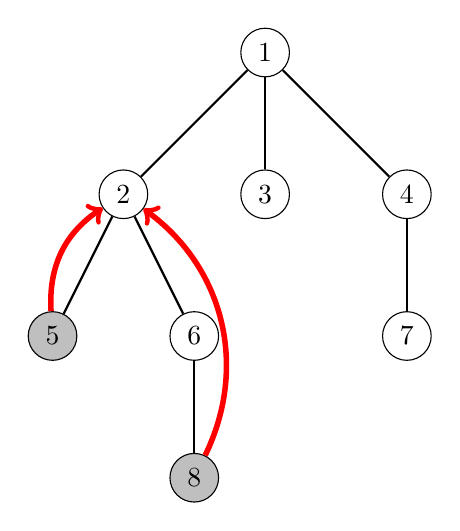
\begin{tikzpicture}[scale=0.9]
\node[draw, circle] (1) at (0,3) {$1$};
\node[draw, circle] (2) at (2,1) {$4$};
\node[draw, circle] (3) at (-2,1) {$2$};
\node[draw, circle] (4) at (0,1) {$3$};
\node[draw, circle] (5) at (2,-1) {$7$};
\node[draw, circle, fill=lightgray] (6) at (-3,-1) {$5$};
\node[draw, circle] (7) at (-1,-1) {$6$};
\node[draw, circle, fill=lightgray] (8) at (-1,-3) {$8$};
\path[draw,thick,-] (1) -- (2);
\path[draw,thick,-] (1) -- (3);
\path[draw,thick,-] (1) -- (4);
\path[draw,thick,-] (2) -- (5);
\path[draw,thick,-] (3) -- (6);
\path[draw,thick,-] (3) -- (7);
\path[draw,thick,-] (7) -- (8);

\path[draw=red,thick,->,line width=2pt] (6) edge [bend left] (3);
\path[draw=red,thick,->,line width=2pt] (8) edge [bend right=40] (3);
\end{tikzpicture}
\end{center}

A seguir, discutiremos duas técnicas eficientes para encontrar o ancestral comum mais baixo de dois nós.

\subsubsection{Método 1}

Uma maneira de resolver o problema é usar o fato de que podemos encontrar eficientemente o $k$-ésimo ancestral de qualquer nó na árvore. Usando isso, podemos dividir o problema de encontrar o ancestral comum mais baixo em duas partes.

Usamos dois ponteiros que apontam inicialmente para os dois nós cujo ancestral comum mais baixo devemos encontrar. Primeiro, movemos um dos ponteiros para cima para que ambos os ponteiros apontem para nós no mesmo nível.

No cenário de exemplo, movemos o segundo ponteiro um nível para cima para que ele aponte para o nó 6, que está no mesmo nível do nó 5:

\begin{center}
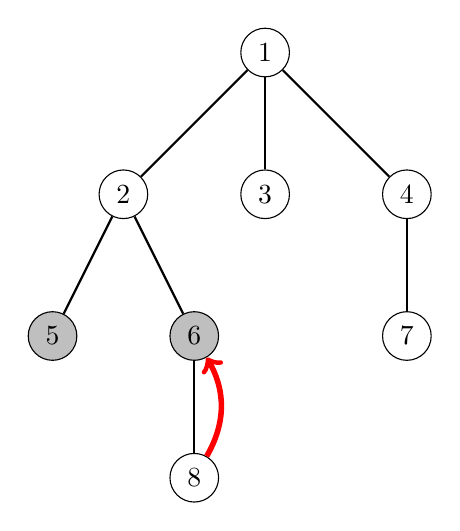
\begin{tikzpicture}[scale=0.9]
\node[draw, circle] (1) at (0,3) {$1$};
\node[draw, circle] (2) at (2,1) {$4$};
\node[draw, circle] (3) at (-2,1) {$2$};
\node[draw, circle] (4) at (0,1) {$3$};
\node[draw, circle] (5) at (2,-1) {$7$};
\node[draw, circle,fill=lightgray] (6) at (-3,-1) {$5$};
\node[draw, circle,fill=lightgray] (7) at (-1,-1) {$6$};
\node[draw, circle] (8) at (-1,-3) {$8$};
\path[draw,thick,-] (1) -- (2);
\path[draw,thick,-] (1) -- (3);
\path[draw,thick,-] (1) -- (4);
\path[draw,thick,-] (2) -- (5);
\path[draw,thick,-] (3) -- (6);
\path[draw,thick,-] (3) -- (7);
\path[draw,thick,-] (7) -- (8);

\path[draw=red,thick,->,line width=2pt] (8) edge [bend right] (7);
\end{tikzpicture}
\end{center}

Depois disso, determinamos o número mínimo de etapas necessárias para mover ambos os ponteiros para cima para que apontem para o mesmo nó. O nó para o qual os ponteiros apontam depois disso é o ancestral comum mais baixo.

No cenário de exemplo, basta mover ambos os ponteiros um passo para cima até o nó 2, que é o ancestral comum mais baixo:

\begin{center}
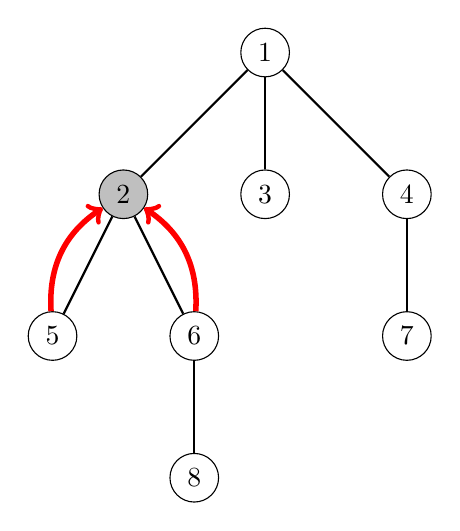
\begin{tikzpicture}[scale=0.9]
\node[draw, circle] (1) at (0,3) {$1$};
\node[draw, circle] (2) at (2,1) {$4$};
\node[draw, circle,fill=lightgray] (3) at (-2,1) {$2$};
\node[draw, circle] (4) at (0,1) {$3$};
\node[draw, circle] (5) at (2,-1) {$7$};
\node[draw, circle] (6) at (-3,-1) {$5$};
\node[draw, circle] (7) at (-1,-1) {$6$};
\node[draw, circle] (8) at (-1,-3) {$8$};
\path[draw,thick,-] (1) -- (2);
\path[draw,thick,-] (1) -- (3);
\path[draw,thick,-] (1) -- (4);
\path[draw,thick,-] (2) -- (5);
\path[draw,thick,-] (3) -- (6);
\path[draw,thick,-] (3) -- (7);
\path[draw,thick,-] (7) -- (8);

\path[draw=red,thick,->,line width=2pt] (6) edge [bend left] (3);
\path[draw=red,thick,->,line width=2pt] (7) edge [bend right] (3);
\end{tikzpicture}
\end{center}

Como ambas as partes do algoritmo podem ser executadas em tempo $O(\log n)$ usando informações pré-calculadas, podemos encontrar o ancestral comum mais baixo de quaisquer dois nós em tempo $O(\log n)$.

\subsubsection{Método 2}

Outra maneira de resolver o problema é baseada em um vetor de percurso de árvore\footnote{Este algoritmo de ancestral comum mais baixo foi apresentado em \cite{ben00}. Essa técnica às vezes é chamada de \index{Euler tour technique}
\key{Euler tour technique} \cite{tar84}.}. Novamente, a ideia é percorrer os nós usando uma busca em profundidade:

\begin{center}
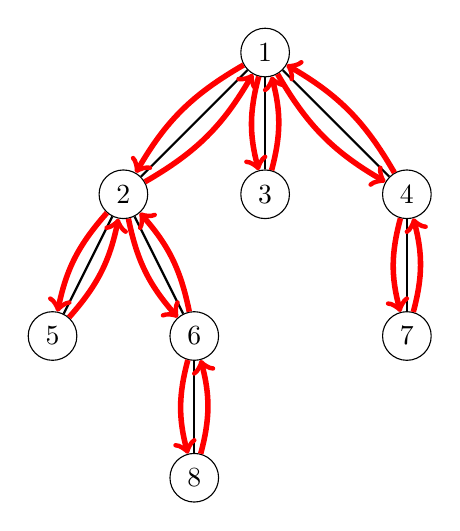
\begin{tikzpicture}[scale=0.9]
\node[draw, circle] (1) at (0,3) {$1$};
\node[draw, circle] (2) at (2,1) {$4$};
\node[draw, circle] (3) at (-2,1) {$2$};
\node[draw, circle] (4) at (0,1) {$3$};
\node[draw, circle] (5) at (2,-1) {$7$};
\node[draw, circle] (6) at (-3,-1) {$5$};
\node[draw, circle] (7) at (-1,-1) {$6$};
\node[draw, circle] (8) at (-1,-3) {$8$};
\path[draw,thick,-] (1) -- (2);
\path[draw,thick,-] (1) -- (3);
\path[draw,thick,-] (1) -- (4);
\path[draw,thick,-] (2) -- (5);
\path[draw,thick,-] (3) -- (6);
\path[draw,thick,-] (3) -- (7);
\path[draw,thick,-] (7) -- (8);

\path[draw=red,thick,->,line width=2pt] (1) edge [bend right=15] (3);
\path[draw=red,thick,->,line width=2pt] (3) edge [bend right=15] (6);
\path[draw=red,thick,->,line width=2pt] (6) edge [bend right=15] (3);
\path[draw=red,thick,->,line width=2pt] (3) edge [bend right=15] (7);
\path[draw=red,thick,->,line width=2pt] (7) edge [bend right=15] (8);
\path[draw=red,thick,->,line width=2pt] (8) edge [bend right=15] (7);
\path[draw=red,thick,->,line width=2pt] (7) edge [bend right=15] (3);
\path[draw=red,thick,->,line width=2pt] (3) edge [bend right=15] (1);
\path[draw=red,thick,->,line width=2pt] (1) edge [bend right=15] (4);
\path[draw=red,thick,->,line width=2pt] (4) edge [bend right=15] (1);
\path[draw=red,thick,->,line width=2pt] (1) edge [bend right=15] (2);
\path[draw=red,thick,->,line width=2pt] (2) edge [bend right=15] (5);
\path[draw=red,thick,->,line width=2pt] (5) edge [bend right=15] (2);
\path[draw=red,thick,->,line width=2pt] (2) edge [bend right=15] (1);
\end{tikzpicture}
\end{center}

No entanto, usamos um vetor de percurso de árvore diferente do que antes: adicionamos cada nó ao vetor \emph{sempre} que a busca em profundidade passa pelo nó, e não apenas na primeira visita. Portanto, um nó que tem $k$ filhos aparece $k+1$ vezes no vetor e há um total de $2n-1$ nós no vetor.

Armazenamos dois valores no vetor: o identificador do nó e a profundidade do nó na árvore. O seguinte vetor corresponde à árvore acima:

\begin{center}
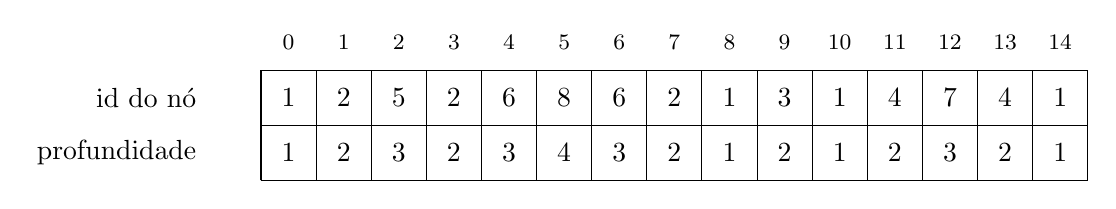
\begin{tikzpicture}[scale=0.7]

\node[left] at (-1,1.5) {id do nó};
\node[left] at (-1,0.5) {profundidade};

\draw (0,1) grid (15,2);
\node at (0.5,1.5) {$1$};
\node at (1.5,1.5) {$2$};
\node at (2.5,1.5) {$5$};
\node at (3.5,1.5) {$2$};
\node at (4.5,1.5) {$6$};
\node at (5.5,1.5) {$8$};
\node at (6.5,1.5) {$6$};
\node at (7.5,1.5) {$2$};
\node at (8.5,1.5) {$1$};
\node at (9.5,1.5) {$3$};
\node at (10.5,1.5) {$1$};
\node at (11.5,1.5) {$4$};
\node at (12.5,1.5) {$7$};
\node at (13.5,1.5) {$4$};
\node at (14.5,1.5) {$1$};

\draw (0,0) grid (15,1);
\node at (0.5,0.5) {$1$};
\node at (1.5,0.5) {$2$};
\node at (2.5,0.5) {$3$};
\node at (3.5,0.5) {$2$};
\node at (4.5,0.5) {$3$};
\node at (5.5,0.5) {$4$};
\node at (6.5,0.5) {$3$};
\node at (7.5,0.5) {$2$};
\node at (8.5,0.5) {$1$};
\node at (9.5,0.5) {$2$};
\node at (10.5,0.5) {$1$};
\node at (11.5,0.5) {$2$};
\node at (12.5,0.5) {$3$};
\node at (13.5,0.5) {$2$};
\node at (14.5,0.5) {$1$};

\footnotesize
\node at (0.5,2.5) {$0$};
\node at (1.5,2.5) {$1$};
\node at (2.5,2.5) {$2$};
\node at (3.5,2.5) {$3$};
\node at (4.5,2.5) {$4$};
\node at (5.5,2.5) {$5$};
\node at (6.5,2.5) {$6$};
\node at (7.5,2.5) {$7$};
\node at (8.5,2.5) {$8$};
\node at (9.5,2.5) {$9$};
\node at (10.5,2.5) {$10$};
\node at (11.5,2.5) {$11$};
\node at (12.5,2.5) {$12$};
\node at (13.5,2.5) {$13$};
\node at (14.5,2.5) {$14$};
\end{tikzpicture}
\end{center}

Agora podemos encontrar o ancestral comum mais baixo dos nós $a$ e $b$ encontrando o nó com a profundidade \emph{mínima} entre os nós $a$ e $b$ no vetor. Por exemplo, o ancestral comum mais baixo dos nós $5$ e $8$ pode ser encontrado da seguinte forma:

\begin{center}
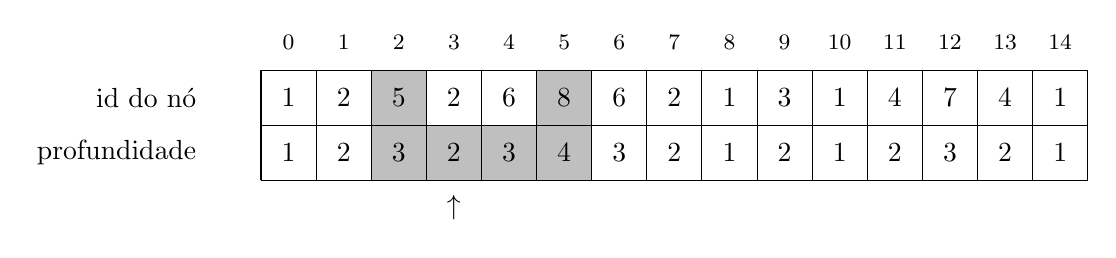
\begin{tikzpicture}[scale=0.7]

\node[left] at (-1,1.5) {id do nó};
\node[left] at (-1,0.5) {profundidade};

\fill[color=lightgray] (2,1) rectangle (3,2);
\fill[color=lightgray] (5,1) rectangle (6,2);
\fill[color=lightgray] (2,0) rectangle (6,1);

\node at (3.5,-0.5) {$\uparrow$};

\draw (0,1) grid (15,2);
\node at (0.5,1.5) {$1$};
\node at (1.5,1.5) {$2$};
\node at (2.5,1.5) {$5$};
\node at (3.5,1.5) {$2$};
\node at (4.5,1.5) {$6$};
\node at (5.5,1.5) {$8$};
\node at (6.5,1.5) {$6$};
\node at (7.5,1.5) {$2$};
\node at (8.5,1.5) {$1$};
\node at (9.5,1.5) {$3$};
\node at (10.5,1.5) {$1$};
\node at (11.5,1.5) {$4$};
\node at (12.5,1.5) {$7$};
\node at (13.5,1.5) {$4$};
\node at (14.5,1.5) {$1$};


\draw (0,0) grid (15,1);
\node at (0.5,0.5) {$1$};
\node at (1.5,0.5) {$2$};
\node at (2.5,0.5) {$3$};
\node at (3.5,0.5) {$2$};
\node at (4.5,0.5) {$3$};
\node at (5.5,0.5) {$4$};
\node at (6.5,0.5) {$3$};
\node at (7.5,0.5) {$2$};
\node at (8.5,0.5) {$1$};
\node at (9.5,0.5) {$2$};
\node at (10.5,0.5) {$1$};
\node at (11.5,0.5) {$2$};
\node at (12.5,0.5) {$3$};
\node at (13.5,0.5) {$2$};
\node at (14.5,0.5) {$1$};

\footnotesize
\node at (0.5,2.5) {$0$};
\node at (1.5,2.5) {$1$};
\node at (2.5,2.5) {$2$};
\node at (3.5,2.5) {$3$};
\node at (4.5,2.5) {$4$};
\node at (5.5,2.5) {$5$};
\node at (6.5,2.5) {$6$};
\node at (7.5,2.5) {$7$};
\node at (8.5,2.5) {$8$};
\node at (9.5,2.5) {$9$};
\node at (10.5,2.5) {$10$};
\node at (11.5,2.5) {$11$};
\node at (12.5,2.5) {$12$};
\node at (13.5,2.5) {$13$};
\node at (14.5,2.5) {$14$};
\end{tikzpicture}
\end{center}

O nó 5 está na posição 2, o nó 8 está na posição 5 e o nó com profundidade mínima entre as posições $2 \ldots 5$ é o nó 2 na posição 3, cuja profundidade é 2. Assim, o ancestral comum mais baixo dos nós 5 e 8 é o nó 2.

Portanto, para encontrar o ancestral comum mais baixo de dois nós, basta processar uma consulta de mínimo de intervalo. Como o vetor é estático, podemos processar tais consultas em tempo $O(1)$ após um pré-processamento de tempo $O(n \log n)$.

\subsubsection{Distâncias entre Nós}

A distância entre os nós $a$ e $b$ é igual ao comprimento do caminho de $a$ para $b$. Acontece que o problema de calcular a distância entre os nós se reduz a encontrar seu ancestral comum mais baixo.

Primeiro, enraizamos a árvore arbitrariamente. Depois disso, a distância dos nós $a$ e $b$ pode ser calculada usando a fórmula
\[\texttt{profundidade}(a)+\texttt{profundidade}(b)-2 \cdot \texttt{profundidade}(c),\]
onde $c$ é o ancestral comum mais baixo de $a$ e $b$ e $\texttt{profundidade}(s)$ denota a profundidade do nó $s$. Por exemplo, considere a distância dos nós 5 e 8:

\begin{center}
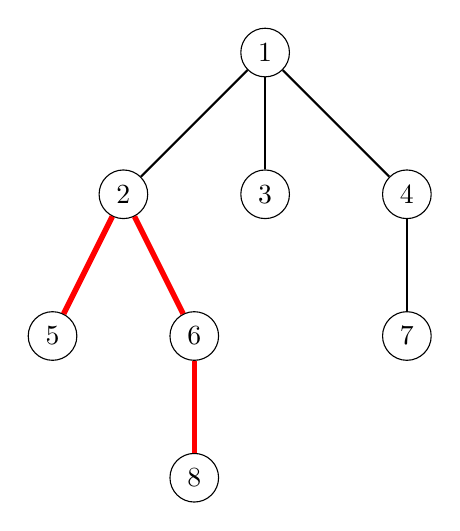
\begin{tikzpicture}[scale=0.9]
\node[draw, circle] (1) at (0,3) {$1$};
\node[draw, circle] (2) at (2,1) {$4$};
\node[draw, circle] (3) at (-2,1) {$2$};
\node[draw, circle] (4) at (0,1) {$3$};
\node[draw, circle] (5) at (2,-1) {$7$};
\node[draw, circle] (6) at (-3,-1) {$5$};
\node[draw, circle] (7) at (-1,-1) {$6$};
\node[draw, circle] (8) at (-1,-3) {$8$};
\path[draw,thick,-] (1) -- (2);
\path[draw,thick,-] (1) -- (3);
\path[draw,thick,-] (1) -- (4);
\path[draw,thick,-] (2) -- (5);
\path[draw,thick,-] (3) -- (6);
\path[draw,thick,-] (3) -- (7);
\path[draw,thick,-] (7) -- (8);

\path[draw=red,thick,-,line width=2pt] (8) -- node[font=\small] {} (7);
\path[draw=red,thick,-,line width=2pt] (7) -- node[font=\small] {} (3);
\path[draw=red,thick,-,line width=2pt] (6) -- node[font=\small] {} (3);
\end{tikzpicture}
\end{center}

O ancestral comum mais baixo dos nós 5 e 8 é o nó 2. As profundidades dos nós são $\texttt{profundidade}(5)=3$, $\texttt{profundidade}(8)=4$ e $\texttt{profundidade}(2)=2$, então a distância entre os nós 5 e 8 é $3+4-2\cdot2=3$.

\section{Algoritmos Offline}

Até agora, discutimos algoritmos \emph{online} para consultas em árvores. Esses algoritmos são capazes de processar consultas uma após a outra, de forma que cada consulta seja respondida antes de receber a próxima consulta.

No entanto, em muitos problemas, a propriedade online não é necessária. Nesta seção, vamos nos concentrar em algoritmos \emph{offline}. Esses algoritmos recebem um conjunto de consultas que podem ser respondidas em qualquer ordem. Muitas vezes, é mais fácil projetar um algoritmo offline em comparação com um algoritmo online.

\subsubsection{Mesclando Estruturas de Dados}

Um método para construir um algoritmo offline é realizar um percurso de árvore em profundidade e manter estruturas de dados nos nós. Em cada nó $s$, criamos uma estrutura de dados $\texttt{d}[s]$ que é baseada nas estruturas de dados dos filhos de $s$. Então, usando esta estrutura de dados, todas as consultas relacionadas a $s$ são processadas.

Como exemplo, considere o seguinte problema: Recebemos uma árvore onde cada nó possui algum valor. Nossa tarefa é processar consultas da forma "calcular o número de nós com valor $x$ na subárvore do nó $s$". Por exemplo, na árvore a seguir, a subárvore do nó $4$ contém dois nós cujo valor é 3.

\begin{center}
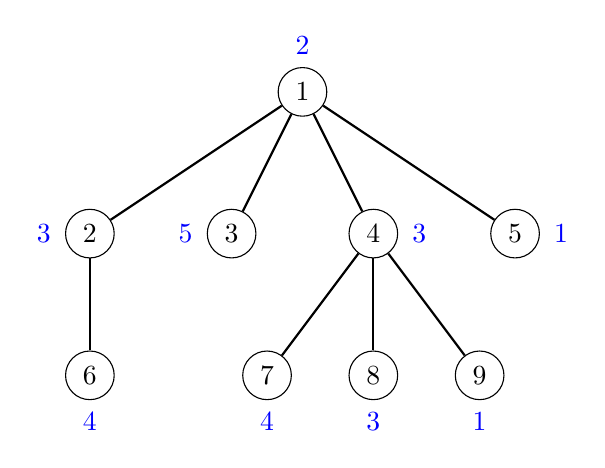
\begin{tikzpicture}[scale=0.9]
\node[draw, circle] (1) at (0,3) {$1$};
\node[draw, circle] (2) at (-3,1) {$2$};
\node[draw, circle] (3) at (-1,1) {$3$};
\node[draw, circle] (4) at (1,1) {$4$};
\node[draw, circle] (5) at (3,1) {$5$};
\node[draw, circle] (6) at (-3,-1) {$6$};
\node[draw, circle] (7) at (-0.5,-1) {$7$};
\node[draw, circle] (8) at (1,-1) {$8$};
\node[draw, circle] (9) at (2.5,-1) {$9$};

\path[draw,thick,-] (1) -- (2);
\path[draw,thick,-] (1) -- (3);
\path[draw,thick,-] (1) -- (4);
\path[draw,thick,-] (1) -- (5);
\path[draw,thick,-] (2) -- (6);
\path[draw,thick,-] (4) -- (7);
\path[draw,thick,-] (4) -- (8);
\path[draw,thick,-] (4) -- (9);

\node[color=blue] at (0,3+0.65) {2};
\node[color=blue] at (-3-0.65,1) {3};
\node[color=blue] at (-1-0.65,1) {5};
\node[color=blue] at (1+0.65,1) {3};
\node[color=blue] at (3+0.65,1) {1};
\node[color=blue] at (-3,-1-0.65) {4};
\node[color=blue] at (-0.5,-1-0.65) {4};
\node[color=blue] at (1,-1-0.65) {3};
\node[color=blue] at (2.5,-1-0.65) {1};
\end{tikzpicture}
\end{center}

Neste problema, podemos usar mapas para responder às consultas. Por exemplo, os mapas para o nó 4 e seus filhos são os seguintes:

\begin{center}
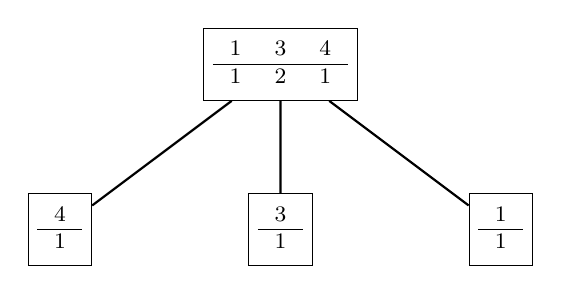
\begin{tikzpicture}[scale=0.7]

\node[draw, rectangle] (a) at (4,5.5)
{
\footnotesize
\begin{tabular}{rrr}
4 \\
\hline
1 \\
\end{tabular}};

\node[draw, rectangle] (b) at (8,5.5)
{
\footnotesize
\begin{tabular}{rrr}
3 \\
\hline
1 \\
\end{tabular}};


\node[draw, rectangle] (c) at (12,5.5)
{
\footnotesize
\begin{tabular}{rr}
1 \\
\hline
1 \\
\end{tabular}};

\node[draw, rectangle] (d) at (8,8.5)
{
\footnotesize
\begin{tabular}{rrr}
1 & 3 & 4 \\
\hline
1 & 2 & 1 \\
\end{tabular}};
\path[draw,thick,-] (a) -- (d);
\path[draw,thick,-] (b) -- (d);
\path[draw,thick,-] (c) -- (d);
\end{tikzpicture}
\end{center}

Se criarmos tal estrutura de dados para cada nó, podemos processar facilmente todas as consultas fornecidas, pois podemos lidar com todas as consultas relacionadas a um nó imediatamente após criar sua estrutura de dados. Por exemplo, a estrutura de mapa acima para o nó 4 nos diz que sua subárvore contém dois nós cujo valor é 3.

No entanto, seria muito lento criar todas as estruturas de dados do zero. Em vez disso, em cada nó $s$, criamos uma estrutura de dados inicial $\texttt{d}[s]$ que contém apenas o valor de $s$. Depois disso, percorremos os filhos de $s$ e \emph{mesclamos} $\texttt{d}[s]$ e todas as estruturas de dados $\texttt{d}[u]$ onde $u$ é um filho de $s$.

Por exemplo, na árvore acima, o mapa para o nó $4$ é criado mesclando os seguintes mapas:

\begin{center}
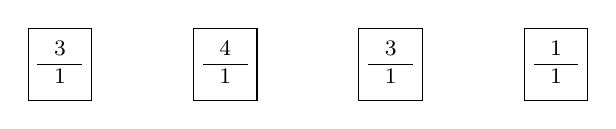
\begin{tikzpicture}[scale=0.7]

\node[draw, rectangle] (a) at (4,5.5)
{
\footnotesize
\begin{tabular}{rrr}
4 \\
\hline
1 \\
\end{tabular}};

\node[draw, rectangle] (b) at (7,5.5)
{
\footnotesize
\begin{tabular}{rrr}
3 \\
\hline
1 \\
\end{tabular}};

\node[draw, rectangle] (c) at (10,5.5)
{
\footnotesize
\begin{tabular}{rr}
1 \\
\hline
1 \\
\end{tabular}};

\node[draw, rectangle] (d) at (1,5.5)
{
\footnotesize
\begin{tabular}{rr}
3 \\
\hline
1 \\
\end{tabular}};

\end{tikzpicture}
\end{center}

Aqui, o primeiro mapa é a estrutura de dados inicial para o nó 4, e os outros três mapas correspondem aos nós 7, 8 e 9.

A mesclagem no nó $s$ pode ser feita da seguinte forma: Percorremos os filhos de $s$ e, em cada filho $u$, mesclamos $\texttt{d}[s]$ e $\texttt{d}[u]$. Sempre copiamos o conteúdo de $\texttt{d}[u]$ para $\texttt{d}[s]$. No entanto, antes disso, \emph{trocamos} o conteúdo de $\texttt{d}[s]$ e $\texttt{d}[u]$ se $\texttt{d}[s]$ for menor que $\texttt{d}[u]$. Ao fazer isso, cada valor é copiado apenas $O(\log n)$ vezes durante o percurso da árvore, o que garante a eficiência do algoritmo.

Para trocar o conteúdo de duas estruturas de dados $a$ e $b$ de forma eficiente, podemos usar o seguinte código:
\begin{lstlisting}
swap(a,b);
\end{lstlisting}
É garantido que o código acima funcione em tempo constante quando $a$ e $b$ são estruturas de dados da biblioteca padrão C++.

\subsubsection{Ancestrais Comuns Mais Baixos}

Há também um algoritmo offline para processar um conjunto de consultas de ancestral comum mais baixo\footnote{Este algoritmo foi publicado por R. E. Tarjan em 1979 \cite{tar79}.}. O algoritmo é baseado na estrutura de dados union-find (consulte o Capítulo 15.2), e o benefício do algoritmo é que ele é mais fácil de implementar do que os algoritmos discutidos anteriormente neste capítulo.

O algoritmo recebe como entrada um conjunto de pares de nós e determina para cada par o ancestral comum mais baixo dos nós. O algoritmo realiza um percurso de árvore em profundidade e mantém conjuntos disjuntos de nós. Inicialmente, cada nó pertence a um conjunto separado. Para cada conjunto, também armazenamos o nó mais alto na árvore que pertence ao conjunto.

Quando o algoritmo visita um nó $x$, ele percorre todos os nós $y$ de forma que o ancestral comum mais baixo de $x$ e $y$ precise ser encontrado. Se $y$ já tiver sido visitado, o algoritmo relata que o ancestral comum mais baixo de $x$ e $y$ é o nó mais alto no conjunto de $y$. Então, após processar o nó $x$, o algoritmo une os conjuntos de $x$ e seu pai.

Por exemplo, suponha que queremos encontrar os ancestrais comuns mais baixos dos pares de nós $(5,8)$ e $(2,7)$ na árvore a seguir:

\begin{center}
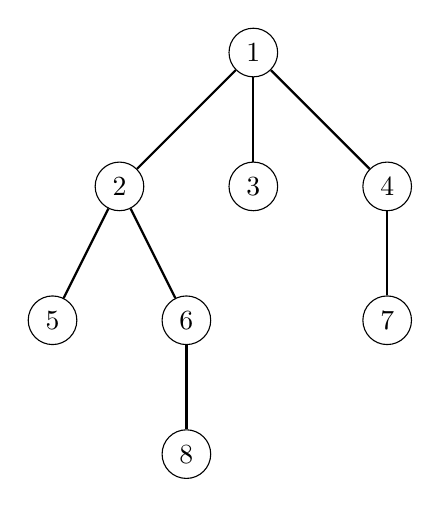
\begin{tikzpicture}[scale=0.85]
\node[draw, circle] (1) at (0,3) {$1$};
\node[draw, circle] (2) at (2,1) {$4$};
\node[draw, circle] (3) at (-2,1) {$2$};
\node[draw, circle] (4) at (0,1) {$3$};
\node[draw, circle] (5) at (2,-1) {$7$};
\node[draw, circle] (6) at (-3,-1) {$5$};
\node[draw, circle] (7) at (-1,-1) {$6$};
\node[draw, circle] (8) at (-1,-3) {$8$};
\path[draw,thick,-] (1) -- (2);
\path[draw,thick,-] (1) -- (3);
\path[draw,thick,-] (1) -- (4);
\path[draw,thick,-] (2) -- (5);
\path[draw,thick,-] (3) -- (6);
\path[draw,thick,-] (3) -- (7);
\path[draw,thick,-] (7) -- (8);
\end{tikzpicture}
\end{center}

Nas árvores a seguir, os nós cinzas denotam nós visitados e grupos de nós tracejados pertencem ao mesmo conjunto. Quando o algoritmo visita o nó 8, ele percebe que o nó 5 foi visitado e o nó mais alto em seu conjunto é 2. Assim, o ancestral comum mais baixo dos nós 5 e 8 é 2:

\begin{center}
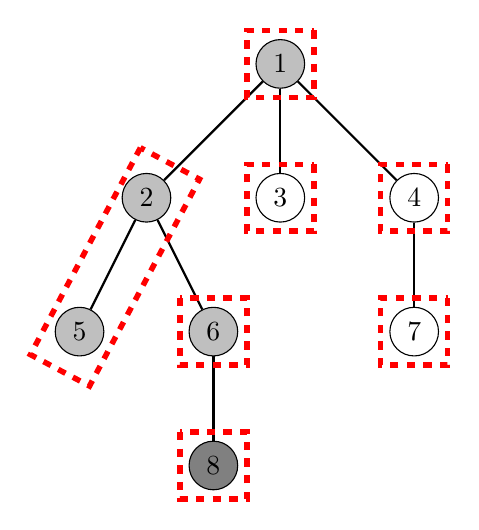
\begin{tikzpicture}[scale=0.85]
\node[draw, circle, fill=lightgray] (1) at (0,3) {$1$};
\node[draw, circle] (2) at (2,1) {$4$};
\node[draw, circle, fill=lightgray] (3) at (-2,1) {$2$};
\node[draw, circle] (4) at (0,1) {$3$};
\node[draw, circle] (5) at (2,-1) {$7$};
\node[draw, circle, fill=lightgray] (6) at (-3,-1) {$5$};
\node[draw, circle, fill=lightgray] (7) at (-1,-1) {$6$};
\node[draw, circle, fill=gray] (8) at (-1,-3) {$8$};
\path[draw,thick,-] (1) -- (2);
\path[draw,thick,-] (1) -- (3);
\path[draw,thick,-] (1) -- (4);
\path[draw,thick,-] (2) -- (5);
\path[draw,thick,-] (3) -- (6);
\path[draw,thick,-] (3) -- (7);
\path[draw,thick,-] (7) -- (8);

\draw [red,thick,dashed,line width=2pt,rotate around={-28:(-2,0)}] (-2.9,1.5) rectangle (-1.9,-2);


\draw [red,thick,dashed,line width=2pt] (-1.5,-0.5) rectangle (-0.5,-1.5);
\draw [red,thick,dashed,line width=2pt] (-1.5,-2.5) rectangle (-0.5,-3.5);

\draw [red,thick,dashed,line width=2pt] (0.5,3.5) rectangle (-0.5,2.5);
\draw [red,thick,dashed,line width=2pt] (0.5,1.5) rectangle (-0.5,0.5);
\draw [red,thick,dashed,line width=2pt] (2.5,1.5) rectangle (1.5,0.5);
\draw [red,thick,dashed,line width=2pt] (2.5,-0.5) rectangle (1.5,-1.5);
\end{tikzpicture}
\end{center}

Mais tarde, ao visitar o nó 7, o algoritmo determina que o ancestral comum mais baixo dos nós 2 e 7 é 1:

\begin{center}
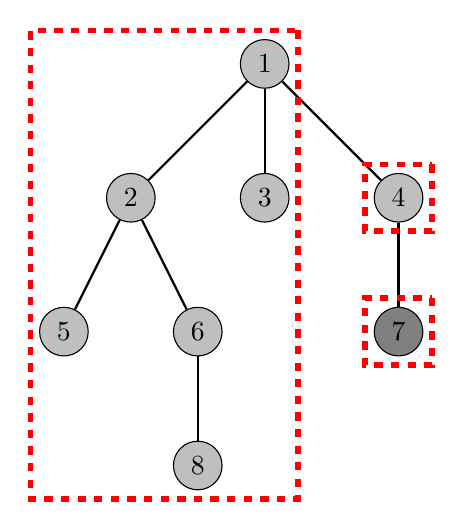
\begin{tikzpicture}[scale=0.85]
\node[draw, circle, fill=lightgray] (1) at (0,3) {$1$};
\node[draw, circle, fill=lightgray] (2) at (2,1) {$4$};
\node[draw, circle, fill=lightgray] (3) at (-2,1) {$2$};
\node[draw, circle, fill=lightgray] (4) at (0,1) {$3$};
\node[draw, circle, fill=gray] (5) at (2,-1) {$7$};
\node[draw, circle, fill=lightgray] (6) at (-3,-1) {$5$};
\node[draw, circle, fill=lightgray] (7) at (-1,-1) {$6$};
\node[draw, circle, fill=lightgray] (8) at (-1,-3) {$8$};
\path[draw,thick,-] (1) -- (2);
\path[draw,thick,-] (1) -- (3);
\path[draw,thick,-] (1) -- (4);
\path[draw,thick,-] (2) -- (5);
\path[draw,thick,-] (3) -- (6);
\path[draw,thick,-] (3) -- (7);
\path[draw,thick,-] (7) -- (8);

\draw [red,thick,dashed,line width=2pt] (0.5,3.5) rectangle (-3.5,-3.5);
\draw [red,thick,dashed,line width=2pt] (2.5,1.5) rectangle (1.5,0.5);
\draw [red,thick,dashed,line width=2pt] (2.5,-0.5) rectangle (1.5,-1.5);

\end{tikzpicture}
\end{center}
